\documentclass[tikz]{standalone}

% arara: pdflatex: { draft: yes }
% arara: pdflatex: { synctex: no }
% arara: latexmk:  { clean: partial }
\begin{document}
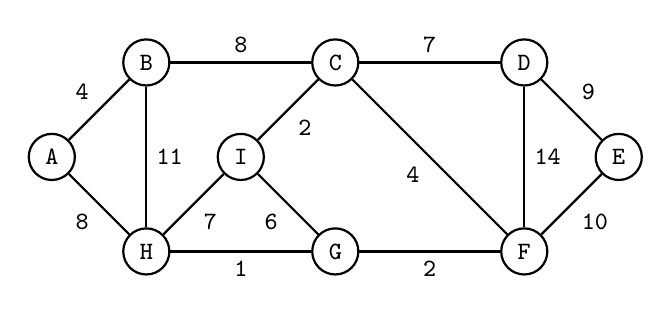
\begin{tikzpicture}[
	% scale=0.73,
	% transform shape,
	thick,
	font=\ttfamily\bfseries\small
]
\tikzset{
    mynode/.style = {circle, draw=black, align=center,fill=white},
    mynodeb/.style = {circle, draw=black, align=center,fill=yellow!40},
    edgen/.style = {-},
    edger/.style = {-,ultra thick,red},
    edgeb/.style = {-,ultra thick,blue},
    edgeg/.style = {-,ultra thick,gray},
}
\node[mynode] at (0.0, 1.2) (a) {A};
\node[mynode] at (1.2, 2.4) (b) {B};
\node[mynode] at (6.0, 2.4) (d) {D};
\node[mynode] at (3.6, 2.4) (c) {C};
\node[mynode] at (1.2, 0.0) (h) {H};
\node[mynode] at (3.6, 0.0) (g) {G};
\node[mynode] at (6.0, 0.0) (f) {F};
\node[mynode] at (2.4, 1.2) (i) {I};
\node[mynode] at (7.2, 1.2) (e) {E};
%
\draw[edgen] (a) edge node[above left] {4} (b);
\draw[edgen] (b) edge node[above] {8} (c);
\draw[edgen] (c) edge node[above] {7} (d);
\draw[edgen] (d) edge node[above right] {9} (e);
%
\draw[edgen] (a) edge node[below left] {8} (h);
\draw[edgen] (h) edge node[below] {1} (g);
\draw[edgen] (g) edge node[below] {2} (f);
\draw[edgen] (f) edge node[below right] {10} (e);
%
\draw[edgen] (h) edge node[below right] {7} (i);
\draw[edgen] (i) edge node[below left] {6} (g);
\draw[edgen] (i) edge node[below right] {2} (c);
%
\draw[edgen] (b) edge node[right] {11} (h);
\draw[edgen] (d) edge node[right] {14} (f);
\draw[edgen] (c) edge node[below left] {4} (f);
\end{tikzpicture}
\end{document}
